\begin{frame}
  \frametitle{Comparativa de Métodos: Implementaciones}

  \begin{table}[h!]
    \centering
    \begin{tabular}{@{}lcc@{}}
      \toprule
      \textbf{Método}       & \texttt{\_predict\_one}                    & \texttt{predict}                      \\ 
      \midrule
      \texttt{QDA}          & Ciclo \texttt{for} por clase              & Ciclo \texttt{for} por observación    \\ 
      \texttt{TensorizedQDA}& Sin ciclos                                & Ciclo \texttt{for} por observación    \\ 
      \texttt{fasterQDA}    & Todo tensorizado                          & Todo tensorizado                      \\ 
      \bottomrule
    \end{tabular}
    \caption{Resumen de las diferencias entre \texttt{QDA}, \texttt{TensorizedQDA} y \texttt{fasterQDA}.}
  \end{table}

\end{frame}

\begin{frame}
  \frametitle{Comparativa de Dimensiones: QDA, TensorizedQDA y fasterQDA}

  \begin{itemize}
    \item X\_unbiased (\(\mathbf{x} - \mu_j)\): Vector de observaciones sin promedios.
    \item Cov\_inv (\(\mathbf{\Sigma_j^{-1}}\)): Matriz de covarianza invertida.
    \item Prod\_int: \((\mathbf{x} - \mu_j)^T \mathbf{\Sigma_j^{-1}} (\mathbf{x} - \mu_j)\).
    \item log\_vero: \( \frac{1}{2} \log{\left|\Sigma_j^{-1}\right|} - \frac{1}{2} (\mathbf{x} - \mu_j)^T \mathbf{\Sigma_j^{-1}} (\mathbf{x} - \mu_j)\).


  \end{itemize}

  \begin{table}[h!]
    \centering
    \begin{tabular}{@{}lcccc@{}}
      \toprule
      \textbf{Método}     		  & X\_unbiased 				 	&Cov\_inv 				 & Prod\_int				& 	 log\_vero		 	 \\ 
      \midrule
      \texttt{QDA}         		 & \(4 \times 1\)              		    & \(4 \times 4\)           		 & \(1\)            			& 	 \cellcolor{yellow}\(1\)				 \\ 
      \texttt{TensorizedQDA}	 & \(3 \times 4 \times 1\)           & \(3 \times 4 \times 4\)     & \(3 \times 1 \)		 	& 	\cellcolor{yellow} \(3 \times 1\)		\\ 
      \texttt{fasterQDA}  	  	 & \(3 \times 4 \times n\)           & \(3 \times 4 \times 4\)     & \(3 \times n \times n\) & 	\cellcolor{yellow}\(3 \times n \) 		\\ 
      \bottomrule
    \end{tabular}
    \caption{Dimensiones de las variables principales por método.}
  \end{table}

  \begin{itemize}
    \item[$\blacktriangleright$] Uso de \texttt{np.diagonal()} para convertir \texttt{Prod\_int} de \(3 \times n \times n\) a \(3 \times n\) en \texttt{log\_vero}.
  \end{itemize}

\end{frame}

\begin{frame}
  \frametitle{Comparativa de Tiempos: QDA, TensorizedQDA y fasterQDA}

  \begin{itemize}
    \item[$\blacktriangleright$] Se utiliza el set de test con un split de 0.3. En este caso, $n=40$
  \end{itemize}

  \begin{table}[h!]
      \centering
      \begin{tabular}{@{}lcc@{}}
        \toprule
        \textbf{Método}      & Tiempo (s)           & Desviación estándar (s) \\ 
        \midrule
        \texttt{QDA}         & 0.00242              & 0.00055                 \\ 
        \texttt{TensorizedQDA} & 0.00062            & 0.00051                 \\ 
        \texttt{fasterQDA}   & 0.00010              & 0.00030                 \\ 
        \bottomrule
      \end{tabular}
      \caption{Tiempos de ejecución de los métodos QDA, TensorizedQDA y FasterQDA.}
  \end{table}

\end{frame}


\begin{frame}
  \frametitle{Comparativa de Tiempos: fasterQDA vs. FasterQDA}

  
  \begin{itemize}
    \item[$\blacktriangleright$] Usando \( \text{diag}(A \cdot B) = \sum_{\text{col}}(A \odot B^T) = \text{np.sum}(A \odot B^T, \text{axis}=1) \) es posible acelerar el método \texttt{fasterQDA}, evitando pasar por la matrices de \( n \times n\).
    \item[$\blacktriangleright$] Se utiliza el set de test con un split de 0.3. En este caso, $n=45$
  \end{itemize}

  \begin{table}[h!]
      \centering
      \begin{tabular}{@{}lcc@{}}
        \toprule
        \textbf{Método}      & Tiempo (s)           & Desviación estándar (s) \\ 
        \midrule
        \texttt{fasterQDA}   & 0.00010              & 0.00030                 \\ 
        \texttt{FasterQDA}   & 0.00008              & 0.00027                 \\ 
        \bottomrule
      \end{tabular}
      \caption{Tiempos de ejecución de los fasterQDA y FasterQDA.}
  \end{table}

\end{frame}


\begin{frame}[fragile]
  \frametitle{Diferencias en el código: fasterQDA vs. FasterQDA}
  \begin{itemize}
    \item[$\blacktriangleright$] Diferencias en los códigos:
  \end{itemize}

  \begin{block}{\texttt{fasterQDA}}
    \begin{lstlisting}[style=pythonstyle]
unbiased_X_transposed =  unbiased_X.transpose(0,2,1) # Forma (classes, n, p)
inner_prod_mat = unbiased_X_transposed @ self.tensor_inv_cov @ unbiased_X # Forma (classes, n, n)
    \end{lstlisting}
  \end{block}
  Costo matemático: \(classes \times (n \times p^2 + n^2 \times p)\)

  \begin{block}{\texttt{FasterQDA}}
    \begin{lstlisting}[style=pythonstyle]
unbiased_X_transposed =  unbiased_X.transpose(0,2,1) # Forma (classes, n, p)
A = unbiased_X_transposed @ self.tensor_inv_cov # Forma (classes, n, p)
inner_prod = (A * unbiased_X_transposed).sum(axis=-1)  # Forma (classes, n)
    \end{lstlisting}
  \end{block}
  Costo matemático: \(classes \times (n \times p^2 + n \times p)\)

\end{frame}


\begin{frame}[fragile]
    \frametitle{Relación en costos matemáticos entre fasterQDA y FasterQDA}
  Comparando, puede verse que la relación en costos entre \texttt{fasterQDA} y \texttt{FasterQDA} es:
  \[
    \frac{classes \times (n \times p^2 + n^2 \times p)}{classes \times (n \times p^2 + n \times p)}
  \]

  \begin{itemize}
    \item[$\blacktriangleright$] Se utiliza el set completo. En este caso, $n=150$
  \end{itemize}

  \begin{table}[h!]
      \centering
      \begin{tabular}{@{}lcc@{}}
        \toprule
        \textbf{Método}      & Tiempo (s)           & Desviación estándar (s) \\ 
        \midrule
        \texttt{fasterQDA}   & 0.00019              & 0.00039                 \\ 
        \texttt{FasterQDA}   & 0.00011              & 0.00032                 \\ 
        \bottomrule
      \end{tabular}
      \caption{Tiempos de ejecución de los fasterQDA y FasterQDA.}
  \end{table}

\end{frame}

\begin{frame}[fragile]
    \frametitle{Speedup de FasterQDA}
\scriptsize
    \begin{itemize}
        \item[$\blacktriangleright$]  En resumen, al evitar la matriz \(n \times n\), \texttt{FasterQDA} logra una aceleración significativa, con un speedup teórico de:
        \[
            \frac{classes \times (n \times p^2 + n^2 \times p)}{classes \times (n \times p^2 + n \times p)} = \frac{n}{p} \quad \text{para} \quad n \gg p
        \]
        \item[$\blacktriangleright$]  Sin embargo, en la práctica, las operaciones adicionales reducen esta aceleración, aunque sigue siendo notable.
    \end{itemize}
    \begin{figure}
        \centering
        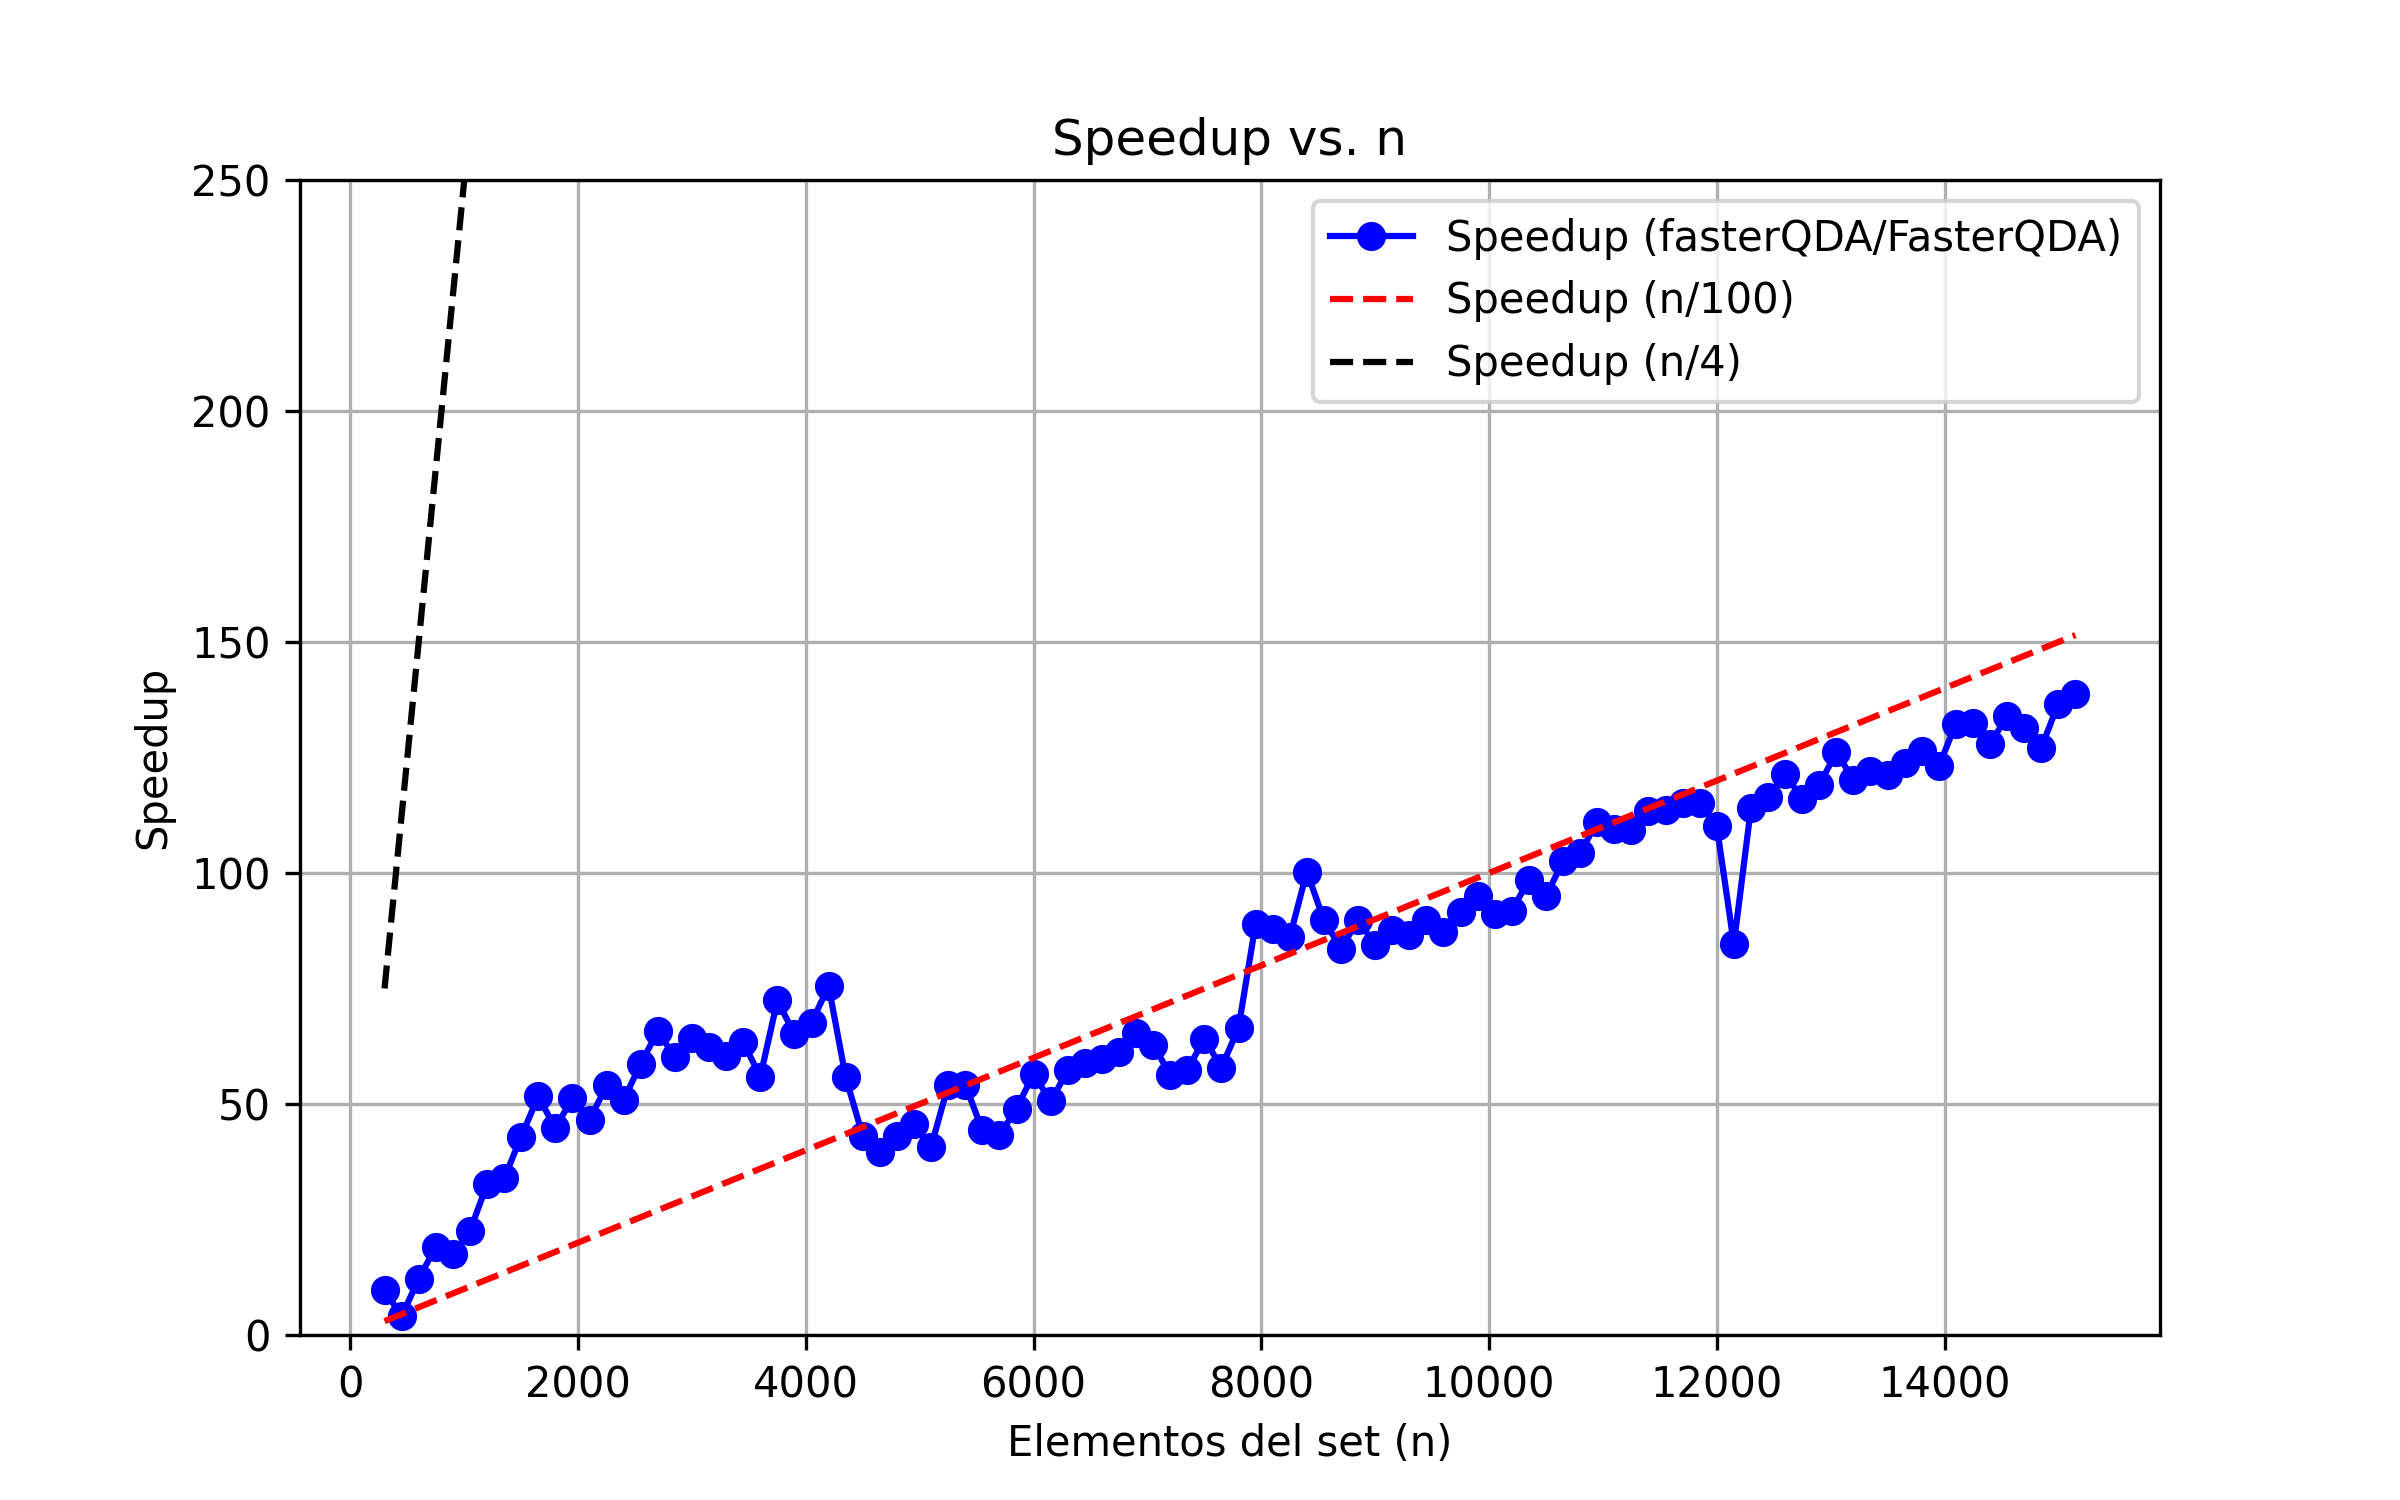
\includegraphics[width=0.6\textwidth]{../speedup_vs_n.png} % Ruta relativa a la imagen
        \caption{Gráfico de Speedup vs. n}
    \end{figure}
\end{frame}
